% =============================================================================
% Supplemental Material — REVTeX 4.2 / PRL format (matches main.tex).
% Converted from the article-class version (preserved in
% supplementary_natcomp_backup.tex). Numeric APS citations (apsrev4-2);
% figures/equations/tables S-prefixed. BUILD ORDER: build both twice so the
% xr-hyper cross-refs between main.tex and supplementary.tex resolve.
% =============================================================================
\documentclass[
    aps,
    prl,
    reprint,
    superscriptaddress,
    amsmath,amssymb,
    nofootinbib,
    floatfix
]{revtex4-2}

\usepackage{graphicx}
\usepackage{bm}
\usepackage{xcolor}
\usepackage[colorlinks=true,allcolors=blue!50!black,citecolor=blue!50!black]{hyperref}
\usepackage{xr-hyper}                             % cross-refs to main-text labels
\externaldocument[M]{main}                            % reads main.aux
\usepackage{lineno}

\graphicspath{{./}{figures/}{SI_figures/}{img/}}

% Supplemental Material numbering (S-prefix)
\renewcommand{\thefigure}{S\arabic{figure}}
\renewcommand{\theequation}{S\arabic{equation}}
\renewcommand{\thetable}{S\arabic{table}}

\begin{document}

\title{Supplemental Material: A temporally-constrained latent space reveals the stochastic dynamics of convective organization}

\author{Sophie Abramian}
\affiliation{Department of Earth and Environmental Engineering, Columbia University, New York, NY, USA}

\author{Olivier Pauluis}
\affiliation{Courant Institute of Mathematical Sciences, New York University, New York, NY, USA}

\author{L. Ruby Leung}
\affiliation{Atmospheric Sciences and Global Change Division, Pacific Northwest National Laboratory, Richland, WA, USA}

\author{Pierre Gentine}
\affiliation{Department of Earth and Environmental Engineering, Columbia University, New York, NY, USA}

\date{\today}

\maketitle
\onecolumngrid   % single-column body (matches main review layout)
\linenumbers

% outline shows section titles only (REVTeX lists starred subsections; suppress them)
\makeatletter
\renewcommand{\l@subsection}[2]{}
\makeatother
\tableofcontents

\newpage

\section{Idealized cloud-resolving simulations}

To examine the response of convection to fixed vertical wind shear, we perform idealized cloud-resolving simulations using the System for Atmospheric Modeling (SAM) \cite{khairoutdinov2003}. Following \cite{muller2013impact}, a low-level shear profile is imposed (see also \cite{rotunno1988theory, houze1977structure, robe2001effect}). The wind profile is linear, with a basal velocity of $8.5\,\mathrm{m\,s^{-1}}$ and a shear depth of $1\,\mathrm{km}$. This value is deliberately suboptimal relative to the shear magnitude ($\sim10\,\mathrm{m\,s^{-1}}$) that maximizes convective organization, in order to enhance sensitivity to internal variability \cite{abramian2022shear}. In this regime, the balance between shear and cold-pool dynamics is more unstable, and variations in cold-pool properties exert a substantial control on convective development.

The model domain spans $128\,\mathrm{km} \times 128\,\mathrm{km}$ horizontally and extends from the surface to $17\,\mathrm{km}$ in the vertical, with enhanced resolution in the boundary layer. A sponge layer is applied near the model top to absorb upward-propagating gravity waves. Microphysical processes are represented using a single-moment scheme. The simulation is first integrated for 30 days to reach radiative--convective equilibrium and then continued for an additional 27 days for analysis. Model output is saved at 2-min intervals, yielding approximately $2\times10^{4}$ time steps, and includes both two- and three-dimensional fields. Under the imposed shear, convection self-organizes into squall-line structures oriented perpendicular to the shear direction (Fig.~\ref{Mfig:simu_isentrop}, main text); the system alternates between quiescent phases and episodes of strong organization, and despite identical large-scale forcing, pronounced variability emerges in the structure, intensity, and persistence of the organized convective systems.

\section{Isentropic mass-flux analysis and preprocessing}

Vertical transport associated with moist convection is inherently three-dimensional, intermittent, and multiscale. When diagnosed directly in physical space, the vertical mass flux reflects the superposition of contributions from convective updrafts and downdrafts, gravity waves, compensating subsidence, and turbulent fluctuations. A physically grounded reduction is provided by isentropic analysis \cite{pauluis2013isentropic}, which conditions transport on thermodynamic variables approximately conserved following moist adiabatic motion \cite{chen2022crucial}. We approximate isentropic surfaces using the moist static energy $h$, and define $h$ and the associated vertical isentropic mass flux as
\begin{align}
    h(x,y,z,t) & = c_p\, T(x,y,z,t)+ g\, z + L_v\, q_v(x,y,z,t),\\
    M(h,z,t) &= \int_{0}^{N_x}\!\!\int_{0}^{N_y} \rho(z,t)\,w(x,y,z,t)\,
    \delta\!\left(\hat{h}(x,y,z,t)-h\right)dx\,dy,
\end{align}
where $c_p$ is the specific heat capacity of air at constant pressure, $T$ is the absolute temperature, $g$ is the gravitational acceleration, $z$ is height, $L_v$ is the latent heat of vaporization, and $q_v$ is the water vapor mixing ratio. The quantity $M(h,z,t)$ is the horizontal integral of the vertical mass flux $\rho w$ projected onto moist static energy levels via the Dirac delta $\delta(\cdot)$; $\rho$ is the air density, $w$ the vertical velocity, $\hat{h}$ the local moist static energy field, and $N_x$, $N_y$ the horizontal domain dimensions. This conditioning reduces dimensionality by collapsing horizontal variability into a compact $(h,z)$ phase space, and separates dynamically distinct processes that overlap in physical space: convective updrafts preferentially transport high-$h$ air upward, evaporatively cooled downdrafts populate lower-$h$ levels, and gravity-wave motions are confined to low-$h$ regions \cite{chen2018atmospheric, chen2020significant, mrowiec2016isentropic}.

The learning dataset is constructed from the time series of isentropic mass-flux fields spanning 27 days at 2-minute resolution. Moist static energy $h$ is discretized into 48 bins from 320 to 350~kJ~kg$^{-1}$, and the vertical coordinate corresponds to the first 48 model levels ($\approx$25~m to 16~km), giving raw dimensions $(n_t \approx 2\times10^{4},\, n_h=48,\, n_z=48)$. For each spatial pixel the temporal mean is removed to isolate transient variability, and a spatial mask retains only pixels nonzero at least once over the time series. A signed logarithmic transform $\mathrm{sign}(x)\,\log(1+|x|)$ enhances weak signals while preserving amplitude ordering. Each training sample consists of a pair $(X_t, X_{t+\Delta t})$ separated by a fixed offset $\Delta t = 5$; the data are randomly permuted and split into training (90\%) and validation (9.9\%) sets, with mini-batches of size 256.

\section{Reduced-order stochastic model}

The reduced-order stochastic model combines a variational autoencoder (VAE), a data-driven latent-state representation, and a discrete-time Markov transition model (Fig.~\ref{Mfig:model}, main text), trained jointly so that the learned latent representation is both physically meaningful and dynamically predictive.

Each isentropic mass-flux diagram $X_t$ is encoded into a $d$-dimensional latent representation by the VAE, whose encoder outputs a diagonal Gaussian posterior $q(z \mid X_t) = \mathcal{N}(\mu(X_t),\,\mathrm{diag}(\sigma^2(X_t)))$. A latent sample $z\sim q(z|X_t)$ (drawn via the reparameterization trick) is decoded to $\hat{X}_t$, with reconstruction enforced through the per-pixel summed squared error $\|X_t-\hat{X}_t\|^2$. The posterior is regularized toward an isotropic prior $p(z)=\mathcal{N}(0,I)$ through the closed-form Kullback--Leibler divergence $D_{\mathrm{KL}}(q\|p) = \tfrac{1}{2}\sum_{i=1}^d(\mu_i^2+\sigma_i^2-\log\sigma_i^2-1)$, entering the objective with a small weight $\beta$.

The continuous latent representation is mapped onto $K=5$ discrete states through a small network with a softmax head, $s_t = \mathrm{softmax}(g(z_t)) \in \Delta^{K-1}$. Because the clustering network is trained jointly with the encoder, it actively reshapes the latent geometry to favour cluster-consistent representations. To prevent state collapse, we regularize the assignment with a contrastive objective $\mathcal{L}_{\mathrm{Dice}}$ based on the structural (Dice) similarity of thresholded isentropic mass-flux anomaly fields: structurally similar pairs are encouraged to share a state, dissimilar pairs to occupy different states (full definition in the contrastive-regularization section below).

Temporal evolution is modeled as a first-order Markov process with row-stochastic transition matrix $T_{ij} = P(s_{t+\Delta t} = j \mid s_t = i)$. The data are sampled every $\Delta t_\text{raw}=2\,\mathrm{min}$, and transitions are evaluated at $\Delta t = 5\,\Delta t_\text{raw} = 10\,\mathrm{min}$. The VAE, state-assignment network, and transition matrix are trained jointly by minimizing a composite objective---reconstruction error, the Kullback--Leibler regularization, the Dice contrastive term $\mathcal{L}_{\mathrm{Dice}}$, and the Markov transition log-likelihood (training objective and curves below)---each weighted by a non-negative coefficient ($\beta$, $\lambda_{\mathrm{Dice}}$, $\gamma_{\mathrm{MC}}$). Optimization uses AdamW (learning rate $5\times10^{-5}$, batch size $256$) for $512$ epochs with gradient-norm clipping at $1.0$; the best model is selected by minimum validation loss.

\section{Training and Validation Losses}


The model is trained for 500 epochs by minimizing a composite objective that combines data fidelity, latent-space regularization, structural contrast, and discrete dynamical consistency. The total loss is given by
\[
\mathcal{L} =
\|X - \hat{X}\|^2
+
\frac{1}{2}\sum_{i=1}^d
\left(
\mu_i^2 + \sigma_i^2 - \log \sigma_i^2 - 1
\right)
-
\mathcal{L}_{\mathrm{Dice}}
-
\sum_{i,j}
s_t(i)\, s_{t+1}(j)\, \log T_{ij},
\]
where the first term corresponds to the reconstruction error, the second term is the Kullback--Leibler divergence enforcing regularization of the continuous latent variables, the third term is a Dice-based contrastive regularization promoting structural separation between latent states, and the final term enforces temporal consistency through a Markov state-transition likelihood.

Figure~\ref{fig:loss_curves} shows the evolution of the total loss and its individual components for both training and validation data. To improve readability, the loss decomposition is shown separately for training and validation. All loss components are displayed on a logarithmic scale to highlight their relative contributions and convergence behavior over the course of training.

The close agreement between training and validation curves across all loss terms indicates stable multi-objective optimization and good generalization, with no evidence of late-epoch overfitting in either the continuous or discrete components of the model.


\begin{figure}
    \centering
    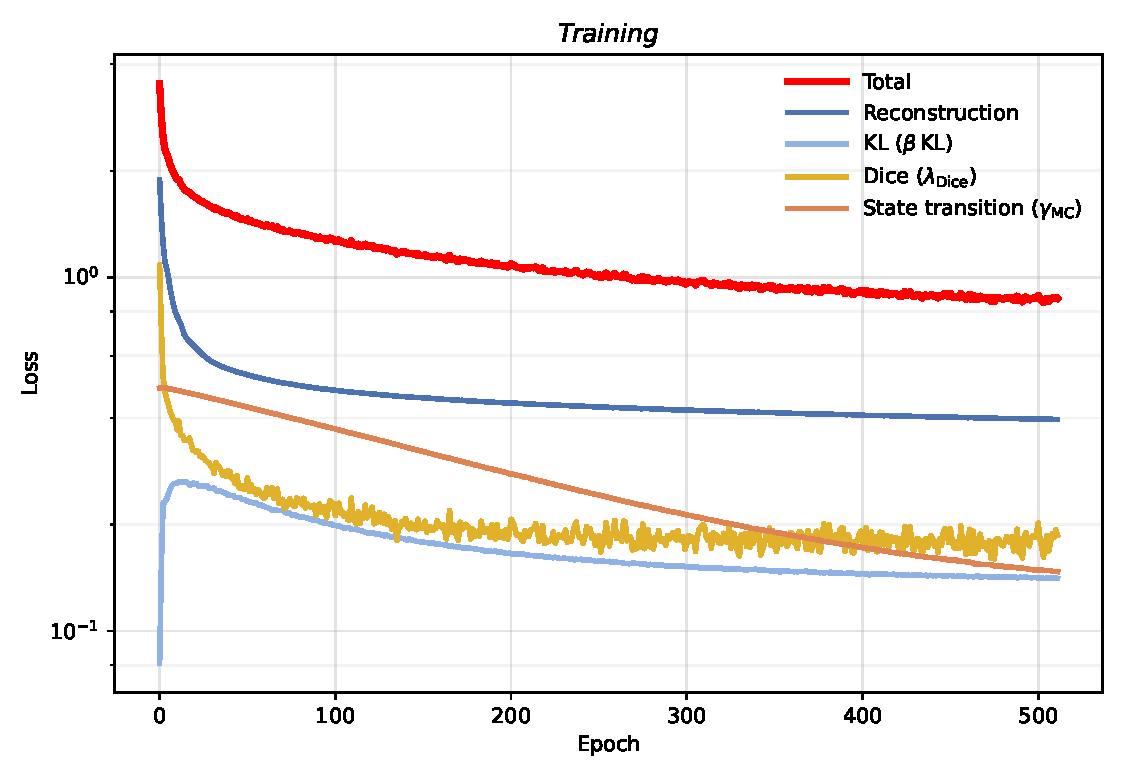
\includegraphics[width=0.49\textwidth]{training_loss.pdf}
    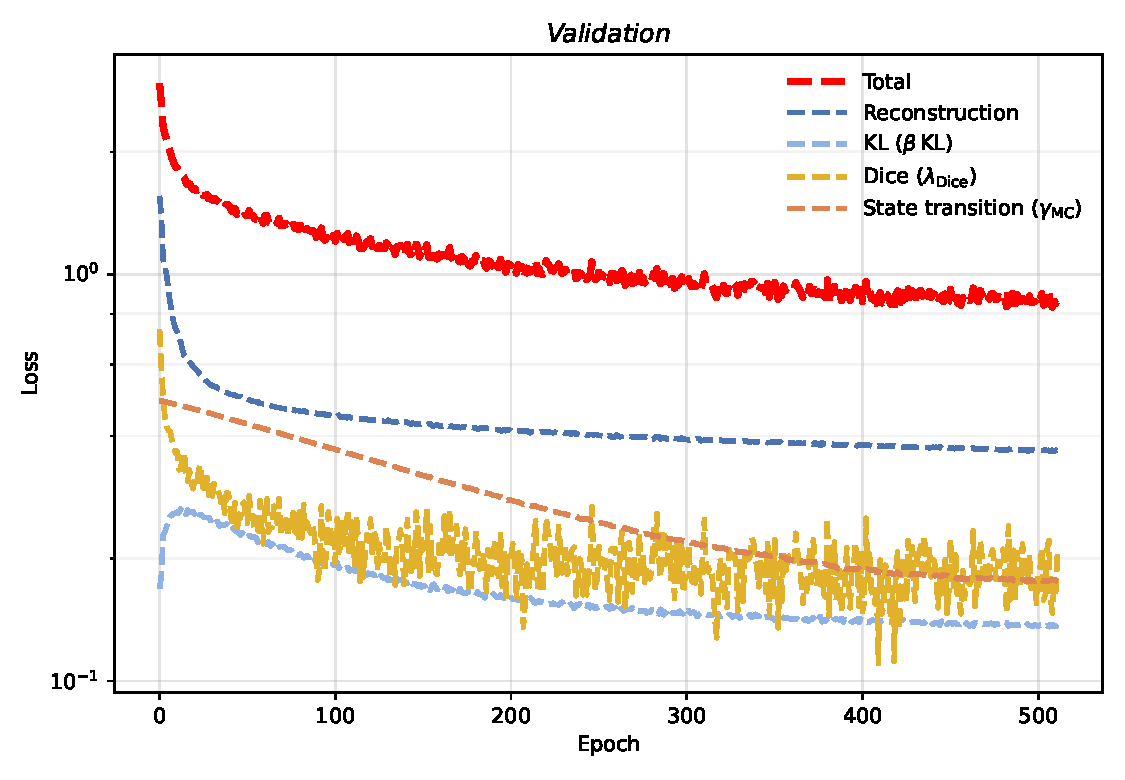
\includegraphics[width=0.49\textwidth]{validation_loss.pdf}
    \caption{Training and validation loss decomposition for the proposed hybrid VAE--Markov model.
Loss components are shown on a logarithmic scale to emphasize their relative magnitudes and convergence behavior across epochs. The consistency between training and validation curves suggests stable optimization and robust generalization across reconstruction, latent regularization, structural contrast, and state-transition dynamics.}
    \label{fig:loss_curves}
\end{figure}



\section{Reconstruction Skills}

To assess the reconstruction capabilities of the model, we show representative examples of reconstructed isentropic mass flux diagrams alongside their corresponding ground-truth fields. Examples are randomly selected from the dataset, with snapshots drawn from different latent states in order to provide an overview of reconstruction performance across the full range of learned dynamical regimes.

For each selected state, a single latent embedding is sampled at random and decoded to produce a reconstructed mass flux field. The reconstructed fields are then compared to the original input fields at the same time index. All examples are displayed using identical color scales to allow direct visual comparison of spatial structure, amplitude, and sign.

As illustrated in Figure~\ref{fig:reconstruction}, the model is able to faithfully recover the dominant spatial patterns and vertical–isentropic structure of the mass flux anomalies across states, while preserving large-scale coherence and sharp gradients. Notably, the reconstructed fields often appear smoother than the corresponding ground-truth inputs, with reduced small-scale variability. This behavior is consistent with the probabilistic nature of variational autoencoders, which tend to suppress high-frequency noise while retaining the most informative components of the signal. Such denoising is indicative of a meaningful and structured latent representation rather than simple memorization of the input fields.

\begin{figure}
    \centering
    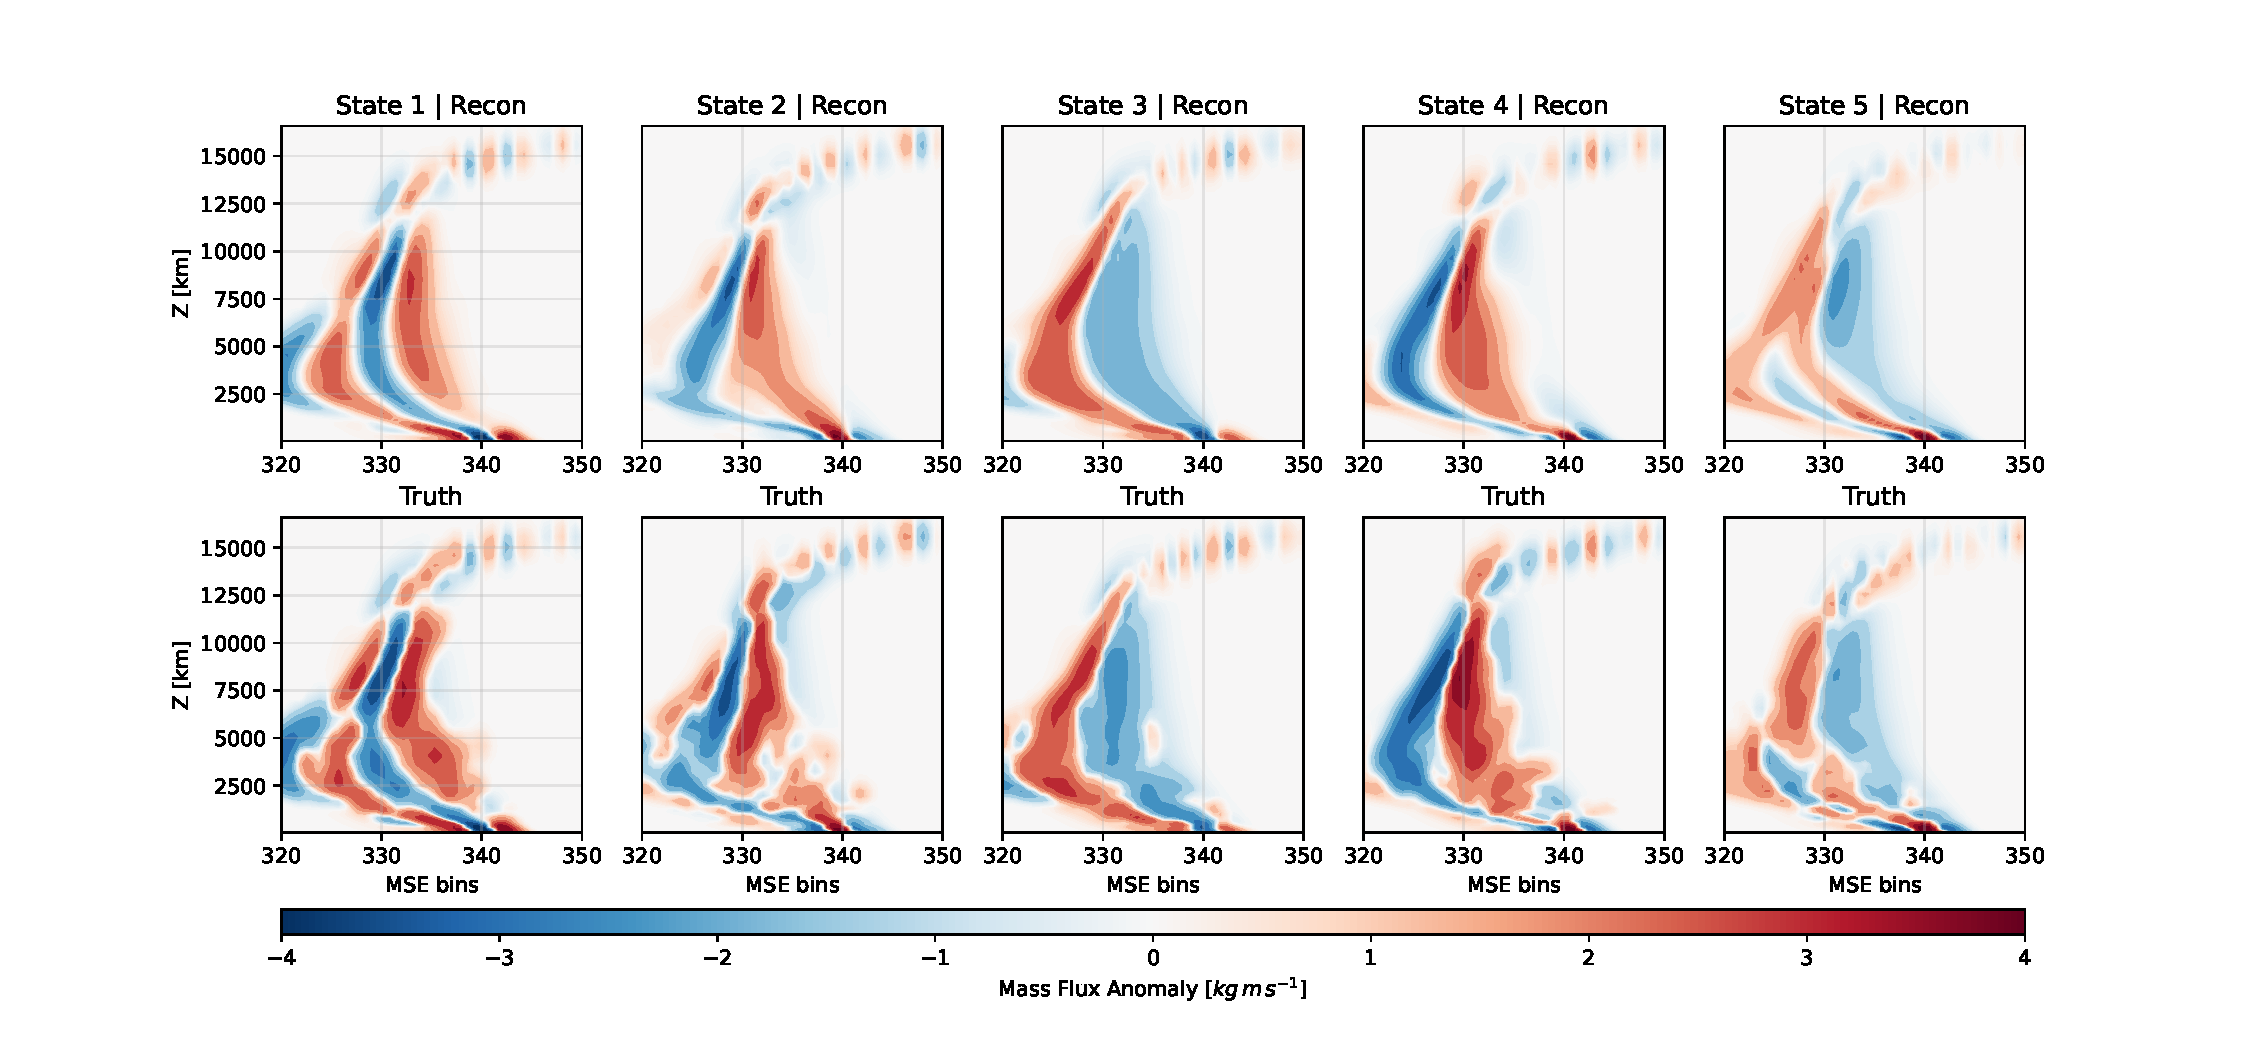
\includegraphics[width=\textwidth]{reconstruction.pdf}
    \caption{Examples of reconstructed and true isentropic mass flux diagrams for randomly selected snapshots from different latent states.
Each column corresponds to a distinct latent state, with one randomly chosen time index per state. The top row shows reconstructions obtained by decoding the latent embedding, while the bottom row shows the corresponding ground-truth fields. All panels use the same color scale, highlighting the model's ability to recover the dominant spatial structure, amplitude, and vertical organization of mass flux anomalies across a range of dynamical regimes.}
    \label{fig:reconstruction}
\end{figure}





\section{Sensitivity test to hyperparameters}
\subsection*{Latent dimension}

We compare the evolution of the reconstruction loss during training for models with different latent dimensionalities equal to 4, 8 (the one chosen) and 16 (Fig.~\ref{fig:latent_dim_sensitivity}). Increasing the latent dimension systematically reduces the reconstruction error and accelerates convergence, reflecting the increased expressive capacity of the latent space. However, beyond a moderate latent size, improvements become marginal, suggesting diminishing returns in reconstruction quality. This supports the choice of an intermediate latent dimension equal to 8 as a trade-off between representational power and model complexity. The logarithmic scale highlights early-epoch differences and stabilisation behaviour across configurations.

\begin{figure}
    \centering
    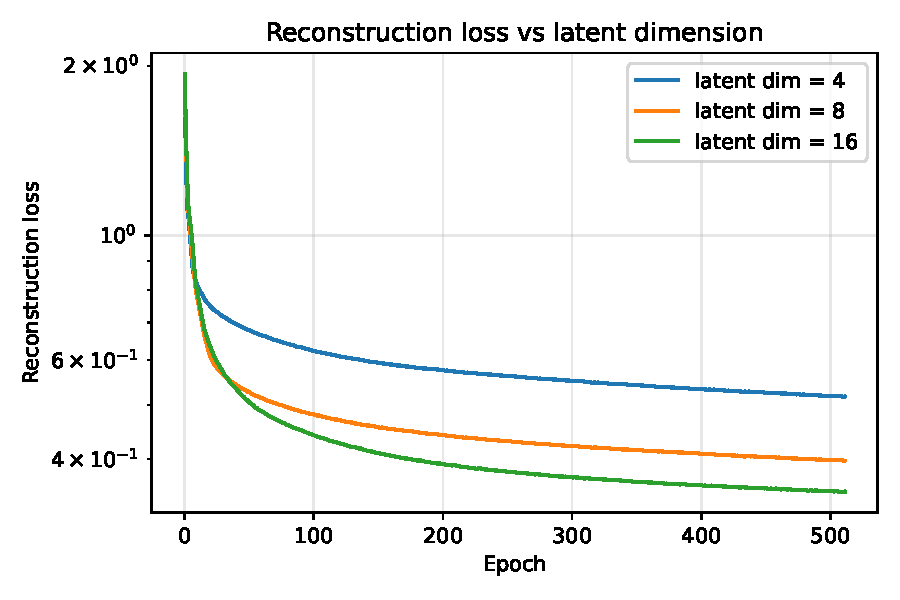
\includegraphics[width=0.7\textwidth]{latent_dim_sensitivity.pdf}
    \caption{Curves show the reconstruction loss as a function of epoch for models with varying latent space sizes. The loss is displayed on a logarithmic scale.}
    \label{fig:latent_dim_sensitivity}
\end{figure}



\subsection*{Number of clusters}

We assess the sensitivity of the latent-space organisation to the prescribed number of discrete clusters by training models with 3, 7, and 10 latent states alongside the 5-state model used in the main text (Fig.~\ref{fig:cluster_sensitivity}). Across all configurations, the separation between organised and unorganised trajectories remains robust, indicating that the inferred dynamical pathways are not an artefact of a particular cluster partitioning. The split is already clearly captured at three clusters: a single organised cluster, a single unorganised cluster, and an intermediate suppressed-convection cluster recover the dominant route through state space. Increasing $K$ to seven or ten refines these regimes into sub-types (multiple sub-organised, dry, or stratiform-leaning sub-clusters) but does not introduce new dynamical regimes; the additional states appear primarily as further subdivisions inside the same two basins. We retain $K=5$ as the working partition because it resolves the two organised regimes (organised-deep Cluster~1 and stratiform-like Cluster~2) and the two unorganised regimes (active-unorganised Cluster~4 and shallow-congestus Cluster~5) without proliferating dynamically redundant sub-states, and because all four headline findings of the main text---the intensity/organisation axis structure, the existence of an organised cluster, the two-regime split carried by the second eigenmode, and the residual non-Markovianity of the organised cluster---survive unchanged across the comparator set.

\begin{figure}
    \centering
    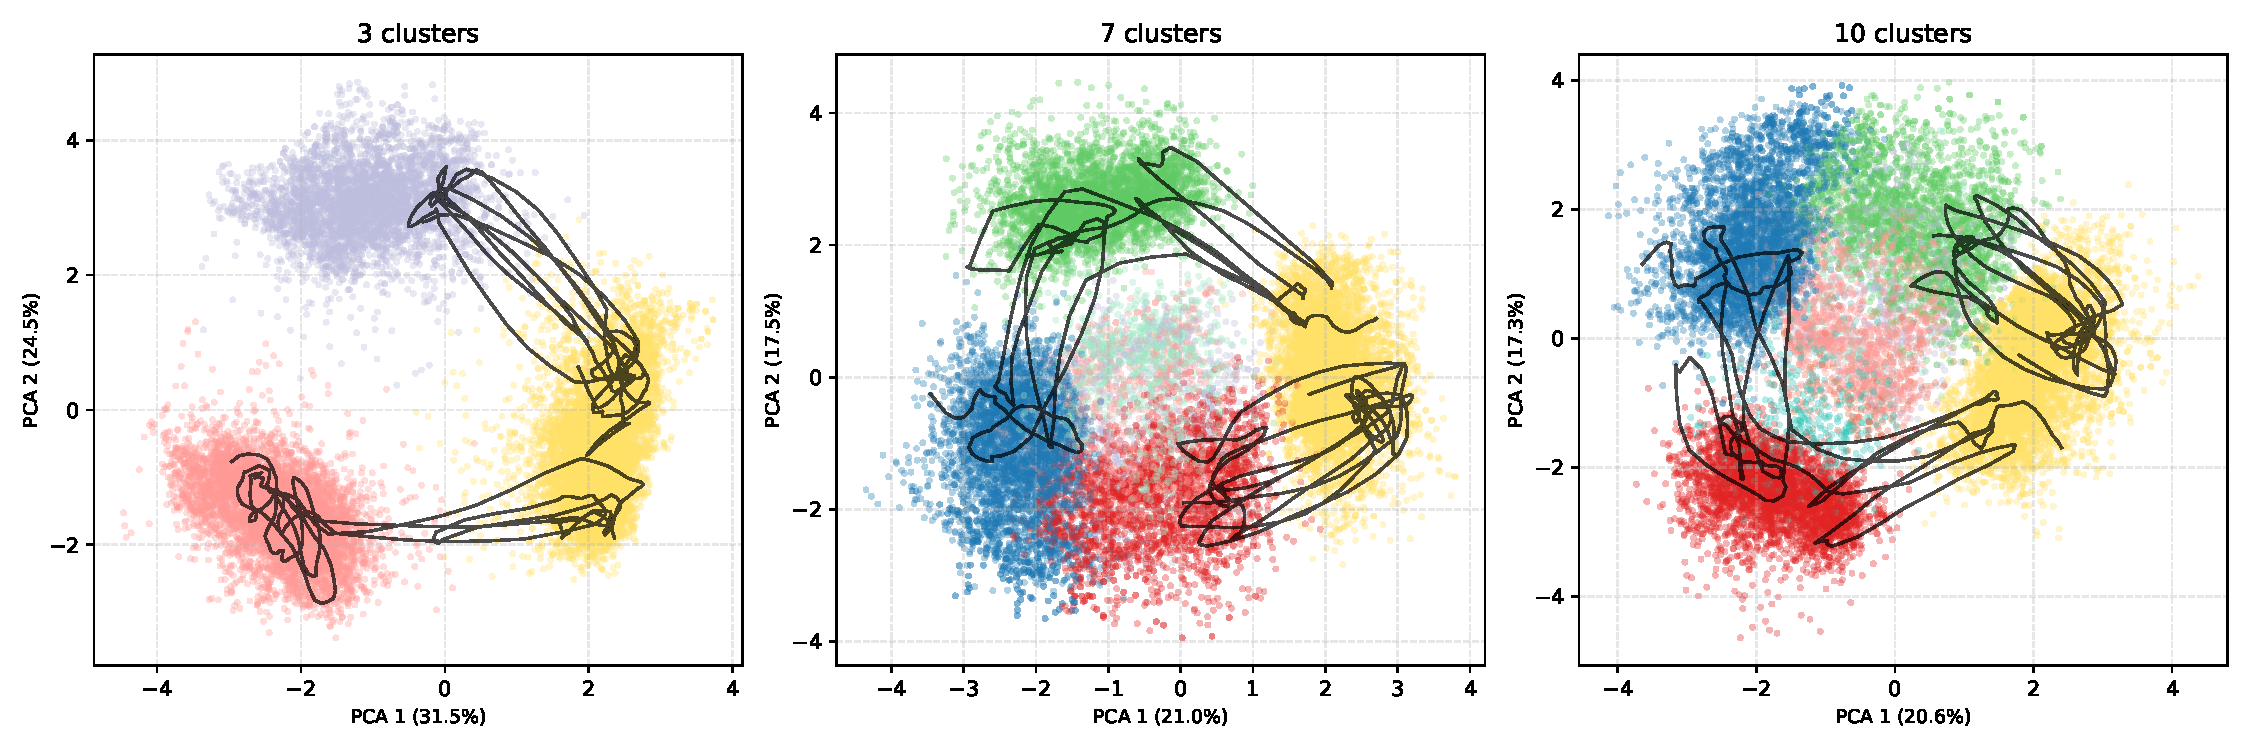
\includegraphics[width=\textwidth]{cluster_sensitivity.pdf}
    \caption{Principal component projections of the latent embeddings for different numbers of discrete latent states.
Panels show the first two principal components of the latent representations for models trained with 3, 7, and 10 clusters (left to right), using a fixed latent dimension of 8. Points are coloured by inferred latent state. Solid black curves indicate smoothed latent-space trajectories from the two representative intervals (strongly organised and weakly organised) used in the main text, allowing the same trajectories to be inspected against each alternative partition.}
    \label{fig:cluster_sensitivity}
\end{figure}

\subsection*{Three-dimensional PCA projection}

The 2D PCA projection in the main text (Fig.~\ref{Mfig:clusters}) suggests partial overlap between some clusters. Expanding to three components shows that clusters which appear to overlap in 2D are separated along higher-order axes (Fig.~\ref{fig:pca_3d}).

\begin{figure}
    \centering
    \IfFileExists{figures/pca_3d.pdf}{%
        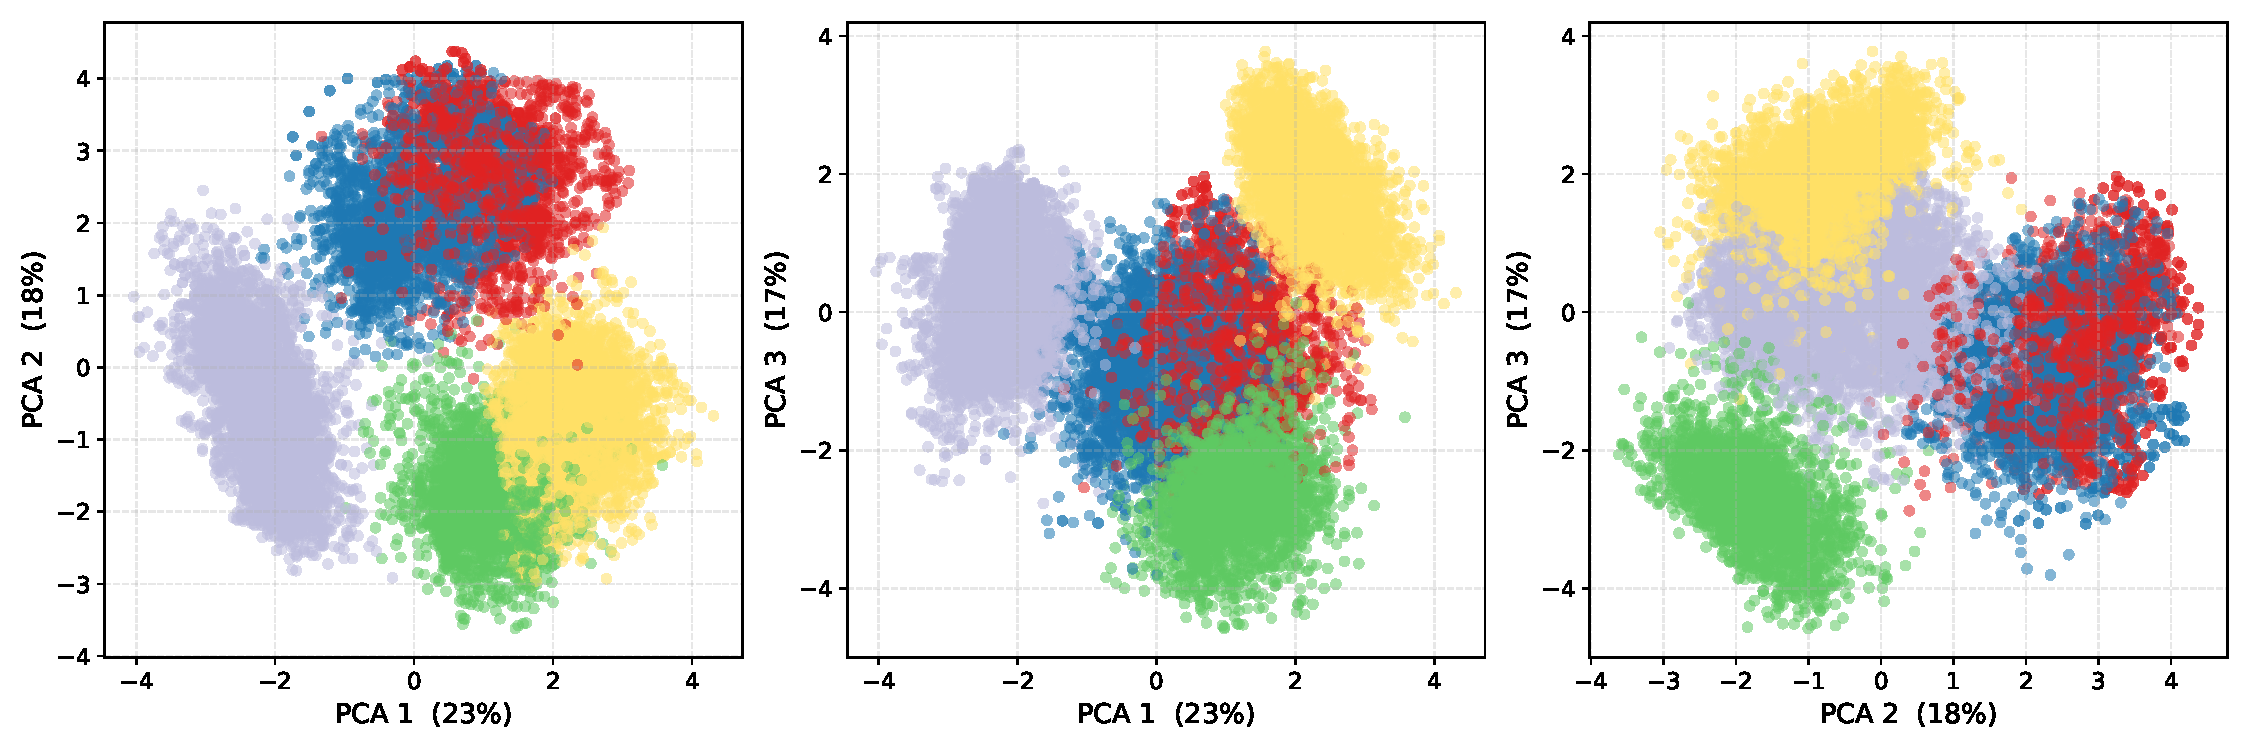
\includegraphics[width=\textwidth]{pca_3d.pdf}%
    }{%
        \framebox[0.6\textwidth]{\parbox[c][4cm][c]{0.55\textwidth}{\centering\itshape
        Figure missing: regenerate \texttt{pca\_3d.pdf} by running \texttt{figures\_si.ipynb}.}}%
    }
    \caption{\textbf{Three-dimensional PCA projection of the latent space.} All three pairwise projections (PCA~1 vs.~PCA~2, PCA~1 vs.~PCA~3, PCA~2 vs.~PCA~3) of the leading three principal components, coloured by latent state. Clusters that appear to overlap in the 2D projection used in the main text are separated along higher-order components.}
    \label{fig:pca_3d}
\end{figure}

\subsection*{Physical interpretation of the latent axes}

The main-text figure colours the PCA projection by state, precipitation, and the PW index. Here we additionally show the joint distributions of the two leading principal components against these diagnostics (Fig.~\ref{fig:axis_var}), which quantify the correlation of PCA~1 with precipitation (intensity) and the anticorrelation of PCA~2 with the variance of precipitable water (organization).

\begin{figure}
    \centering
    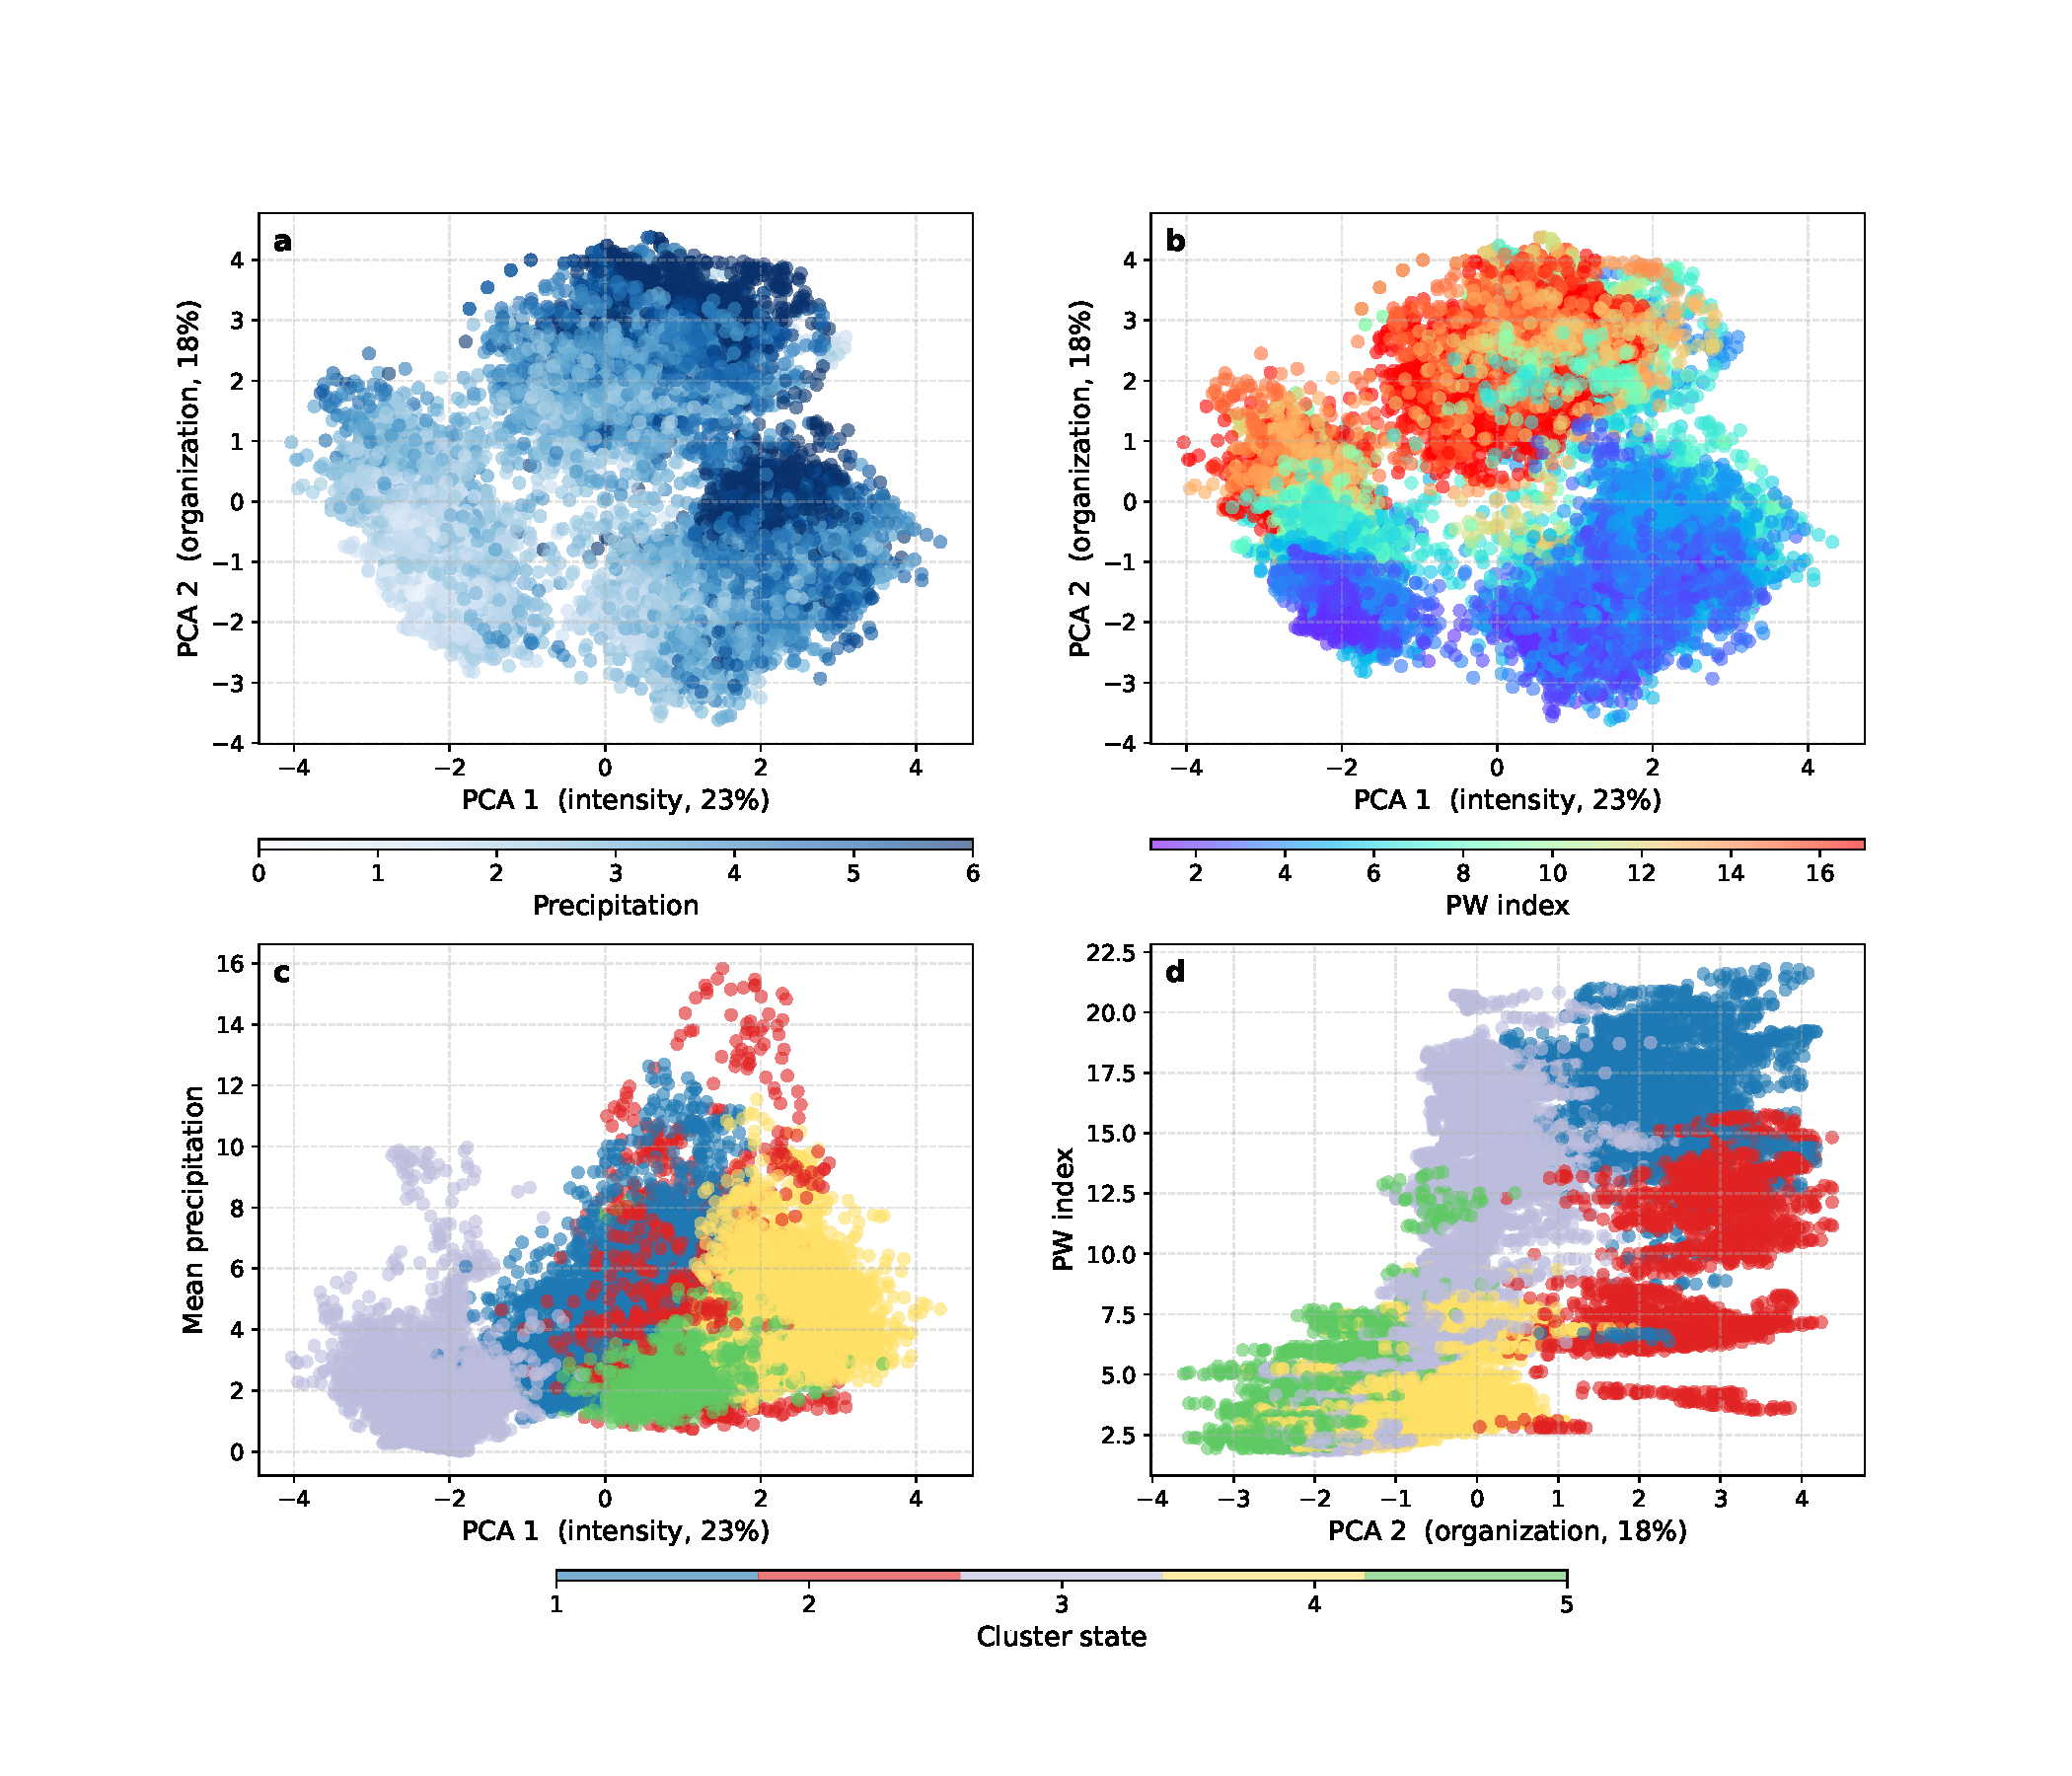
\includegraphics[width=\textwidth]{fig4_latent_axis.pdf}
    \caption{\textbf{Physical interpretation of latent variability.} \textbf{(A)}~PCA projection coloured by the domain-mean precipitation, interpreted as a proxy for the intensity stage of the convective life cycle. \textbf{(B)}~PCA projection coloured by the variance of precipitable water (PW) over the domain, interpreted as a proxy for the spatial organization of the convective field: higher var(PW) corresponds to more clustered, organized convection. \textbf{(C--D)}~Joint distributions of the first two principal components against, respectively, the mean precipitation and the variance of PW.}
    \label{fig:axis_var}
\end{figure}


\section{Contrastive regularization of state assignments}

To regularize the latent state assignment and prevent state collapse, we introduce a contrastive loss that enforces consistency between discrete state probabilities and the structural similarity of the underlying mass-flux anomaly fields.

\paragraph{Structural similarity.}
Given a sample $i$ with reconstructed mass-flux anomaly field $x_i(\mathbf{r})$, we define a discrete structural representation by thresholding the field into three classes using fixed values $\{-1.5,\,1.5\}$:
\[
m_i(\mathbf{r}) =
\begin{cases}
0, & x_i(\mathbf{r}) < -1.5, \\
1, & -1.5 \le x_i(\mathbf{r}) \le 1.5, \\
2, & x_i(\mathbf{r}) > 1.5.
\end{cases}
\]
For each class $c \in \{0,1,2\}$, we define the corresponding binary mask
\[
M_i^c(\mathbf{r}) = \mathbf{1}\!\left[m_i(\mathbf{r}) = c\right].
\]

The structural similarity between two samples $i$ and $j$ is quantified using a macro-averaged Dice coefficient,
\[
\mathrm{Dice}(i,j)
=
\frac{1}{3}
\sum_{c=0}^{2}
\frac{2\,|M_i^c \cap M_j^c|}{|M_i^c| + |M_j^c|},
\]
with the convention that the Dice score for class $c$ is set to $1$ when both masks are empty. We define the corresponding Dice distance as
\[
d_{ij} = 1 - \mathrm{Dice}(i,j),
\]
so that $d_{ij} \in [0,1]$, with small values indicating high structural similarity.

\paragraph{Probabilistic state agreement.}
Let $s_i \in \mathbb{R}^K$ denote the soft state assignment for sample $i$, where $s_i(k)$ is the probability of occupying state $k$. The probability that two samples share the same state is defined as
\[
p_{\mathrm{same}}(i,j) = \sum_{k=1}^K s_i(k)\, s_j(k),
\qquad
p_{\mathrm{diff}}(i,j) = 1 - p_{\mathrm{same}}(i,j).
\]

\paragraph{Soft contrastive windows.}
We distinguish three regimes based on the Dice distance $d_{ij}$: a cohesion regime for structurally similar pairs, a separation regime for dissimilar pairs, and an intermediate regime. These regimes are implemented using linear soft windows with thresholds $\tau_{\mathrm{coh}}$ and $\tau_{\mathrm{sep}}$ and width parameter $w$:
\[
w_{\mathrm{coh}}(d_{ij}) =
\mathrm{clip}\!\left(\frac{\tau_{\mathrm{coh}} - d_{ij}}{w},\,0,\,1\right),
\]
\[
w_{\mathrm{sep}}(d_{ij}) =
\mathrm{clip}\!\left(\frac{d_{ij} - \tau_{\mathrm{sep}}}{w},\,0,\,1\right),
\]
\[
w_{\mathrm{mid}}(d_{ij}) =
\mathrm{clip}\!\left(\frac{d_{ij} - \tau_{\mathrm{coh}}}{w},\,0,\,1\right)
\cdot
\mathrm{clip}\!\left(\frac{\tau_{\mathrm{sep}} - d_{ij}}{w},\,0,\,1\right).
\]

\paragraph{Pairwise penalties.}
For each sampled pair $(i,j)$, we define three complementary penalties:
\begin{itemize}
\item \textbf{Cohesion penalty} (similar structures assigned to different states):
\[
\mathcal{L}_{\mathrm{coh}}(i,j)
=
w_{\mathrm{coh}}(d_{ij}) \, \bigl(1 - p_{\mathrm{same}}(i,j)\bigr),
\]
\item \textbf{Separation penalty} (dissimilar structures assigned to the same state):
\[
\mathcal{L}_{\mathrm{sep}}(i,j)
=
w_{\mathrm{sep}}(d_{ij}) \, p_{\mathrm{same}}(i,j),
\]
\item \textbf{Mid-range uncertainty penalty} (ambiguous similarity with uncertain assignment):
\[
\mathcal{L}_{\mathrm{mid}}(i,j)
=
\lambda_{\mathrm{mid}}\,
w_{\mathrm{mid}}(d_{ij})\,
p_{\mathrm{same}}(i,j)\, p_{\mathrm{diff}}(i,j),
\]
where $\lambda_{\mathrm{mid}}$ controls the strength of the uncertainty penalty.
\end{itemize}

\paragraph{Final contrastive loss.}
The total Dice-based contrastive loss is obtained by averaging over a set $\mathcal{P}$ of randomly sampled pairs within each batch:
\[
\mathcal{L}_{\mathrm{Dice}}
=
\frac{1}{|\mathcal{P}|}
\sum_{(i,j)\in\mathcal{P}}
\Bigl(
\mathcal{L}_{\mathrm{coh}}(i,j)
+
\mathcal{L}_{\mathrm{sep}}(i,j)
+
\mathcal{L}_{\mathrm{mid}}(i,j)
\Bigr).
\]

This loss enforces that latent states correspond to consistent spatial structures of positive and negative mass-flux anomalies, while avoiding degenerate solutions in which all samples collapse onto a single state. Importantly, the loss operates purely on structural information and does not constrain anomaly amplitude or fine-scale intensity.


\section{Markov Chain and the Koopman operator}

The Markov transition model introduced above naturally emerges from the framework of Koopman operator theory, which provides a linear, generally infinite-dimensional, representation of nonlinear dynamical systems by acting on observables---functions of the system state---rather than on the state variables themselves.

Let $x_t \in \mathcal{X}$ denote the full convective state of the system at time $t$. We approximate the Koopman observable with a universal function approximator: a VAE-based neural network, which maps each convective snapshot to a latent representation $z_t = E(x_t)$ and subsequently to a probability vector
\[
\pi(x_t) = (\pi_1(x_t), \ldots, \pi_K(x_t)) \in \Delta^{K-1},
\]
where $\pi_i(x_t) = \mathbb{P}(s_t = i \mid x_t)$ denotes the probability of assignment to convective state $i$. The components of $\pi$ thus define a finite set of learned, smooth observables $f_i = \pi_i \circ E$, parameterized by the VAE encoder $E$.

Under the assumption that the evolution of these observables is approximately Markovian, the Koopman operator $\mathcal{K}$ acts on an observable $f$ according to
\[
(\mathcal{K} f)(x_t) = \mathbb{E}\!\left[ f(x_{t+1}) \mid x_t \right].
\]
Restricting $\mathcal{K}$ to the finite-dimensional subspace spanned by $\{ f_i \}_{i=1}^K$, its action is approximated by a stochastic transition matrix $T$, such that
\[
\mathbb{E}\!\left[ \pi(x_{t+1}) \mid \pi(x_t) \right] \;\approx\; T \, \pi(x_t),
\]
where $T$ represents the action of the stochastic Koopman operator projected onto the subspace defined by the VAE-learned observables.

The spectral properties of $T$ provide insight into the intrinsic dynamics of the reduced system. The leading eigenvalue $\lambda_1 = 1$ corresponds to the stationary distribution over convective states, while subdominant eigenvalues characterize slowly decaying modes associated with regime persistence and long-lived correlations. Complex-conjugate eigenvalue pairs indicate oscillatory behavior or preferred cyclic transition pathways in the reduced state space.

This formulation establishes a principled connection between the VAE-based universal approximation of Koopman observables and data-driven stochastic modeling of convective variability, enabling the identification of dominant regimes, transition pathways, and intrinsic time scales of convective organization.

Time series of individual realizations confirm that system trajectories cluster along the two dominant pathways identified from the leading eigenmode of $T$ (Fig.~\ref{fig:trajectories}); these are the same trajectories overlaid on the latent space in the main text.

\begin{figure}
    \centering
    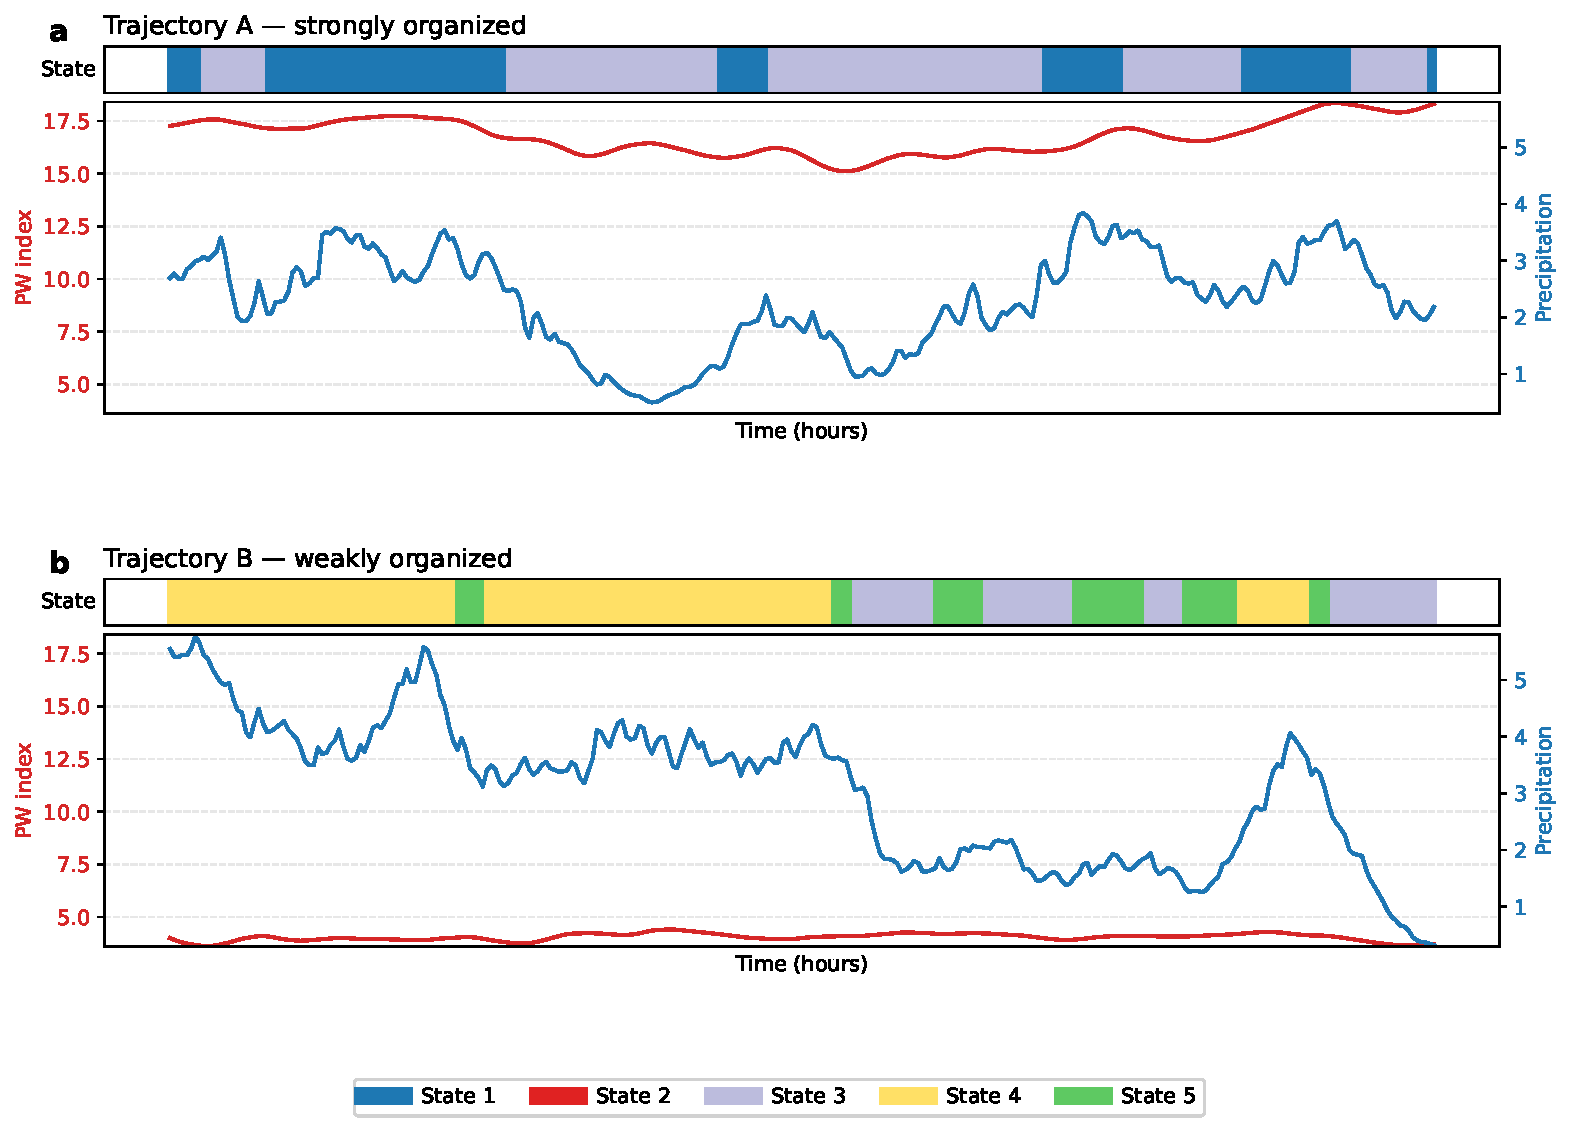
\includegraphics[width=\textwidth]{fig8_trajectories.pdf}
    \caption{\textbf{Example trajectories.} Domain-wide precipitable water (blue, left axis) and precipitation (red, right axis) over two 10-hour intervals, with the latent state at each time step indicated by the colored stripe above each panel. \textbf{(a)} Strongly-organized pathway. \textbf{(b)} Weakly-organized pathway.}
    \label{fig:trajectories}
\end{figure}

\section{Per-state mass-flux profiles}

Let $M(h,z,t)$ denote the isentropic mass flux at time $t$, height $z$, and moist static energy $h$. For each cluster $c$, we define the cluster-mean vertically integrated positive and negative mass fluxes,
\begin{equation}
M^{\pm}_c(z)
=
\left\langle
\int_h M(h,z,t)\,\mathbf{1}\{\pm M>0\}
\right\rangle_{t\in c},
\end{equation}
and the anomalies relative to the simulation-wide mean profiles $\overline{M}^{\pm}(z)$,
\begin{equation}
\Delta^{\pm}_c(z)
=
M^{\pm}_c(z)-\overline{M}^{\pm}(z).
\end{equation}

% --- Per-cluster vertical-profile description ---
The resulting vertical profiles (Fig.~\ref{fig:vertical_profiles}) reveal sharp dynamical distinctions between states. State~1 shows a positive (upward) anomaly extending through the deep troposphere with a comparatively weak negative (downward) anomaly at low levels, consistent with sustained deep ascent in a moist environment that suppresses lower-tropospheric detrainment. State~2 shows an even stronger upper-tropospheric positive anomaly together with the deepest negative anomaly at mid-levels, the signature of a mature mesoscale-stratiform precipitation-driven system. State~3 shows weak anomalies of either sign throughout the column. State~4 shows strong positive and negative anomalies that peak at lower altitudes than Clusters~1--2, characteristic of active but weakly organized convection. State~5 carries small positive anomalies confined to the lower troposphere over an otherwise weak deep-column signal, consistent with residual shallow convection in a suppressed environment.

\begin{figure}[t]
    \centering
    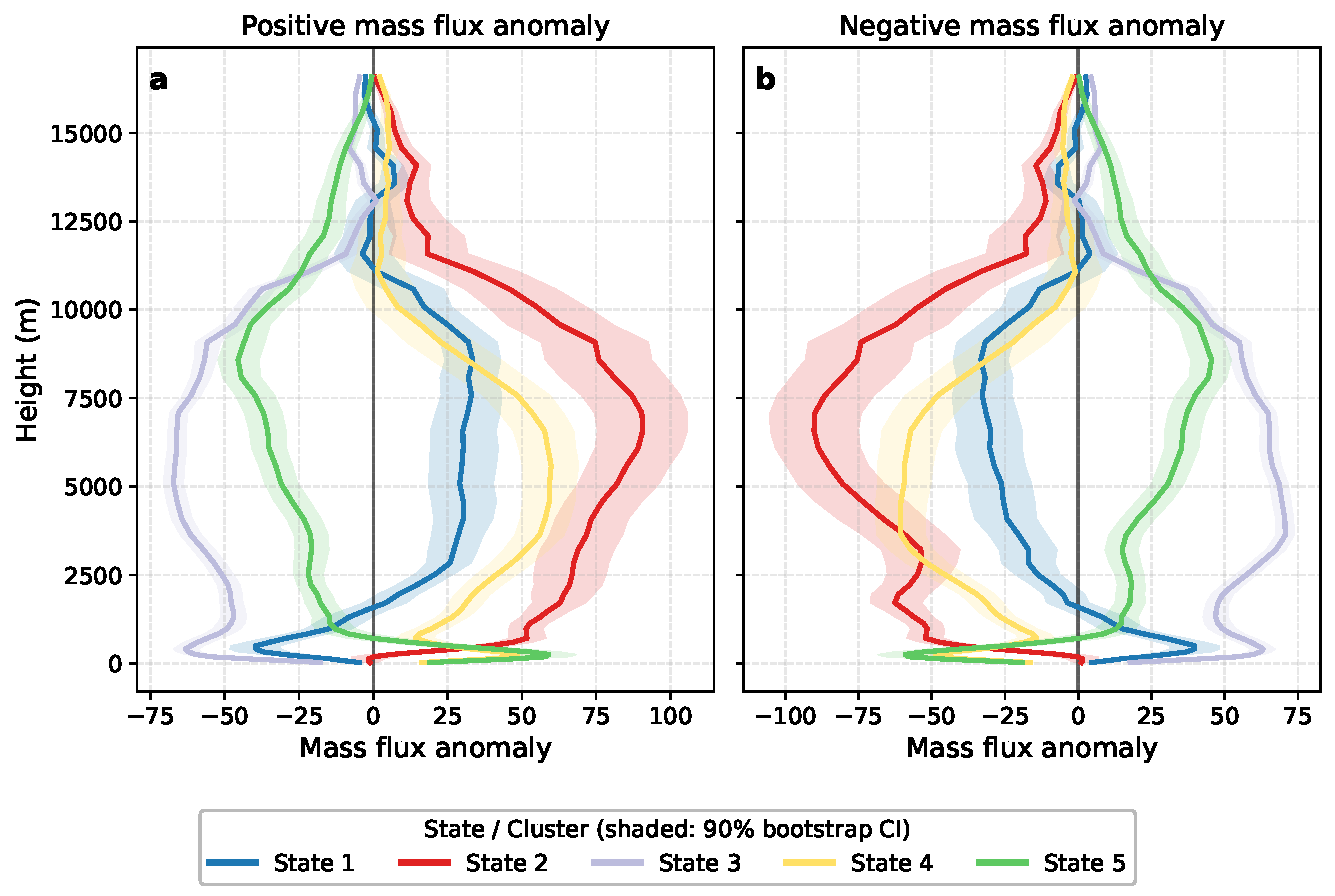
\includegraphics[width=0.72\textwidth]{fig5_vertical_profiles.pdf}
    \caption{\textbf{State-averaged vertical mass-flux anomalies.} \textbf{(a)}~Positive (upward) and \textbf{(b)}~negative (downward) vertically resolved mass-flux anomalies relative to the simulation-wide mean profile $\overline{M}^{\pm}(z)$, computed from the samples closest to each state centroid in latent space. Each colour corresponds to one state (see legend); solid lines indicate the per-cluster mean, and shaded bands show the 90\% bootstrap confidence interval. A positive value at altitude $z$ means the cluster's upward (or downward) mass flux at that height exceeds the simulation-wide mean; a negative value means it lies below.}
    \label{fig:vertical_profiles}
\end{figure}

% --- Per-cluster moist-static-energy description ---
The distribution of mass-flux anomalies across moist static energy (Fig.~\ref{fig:mse_profiles}) reveals corresponding thermodynamic distinctions. State~1 carries its strongest positive (upward) anomaly at high moist static energy ($\theta \approx 343$~K), consistent with the lifting of warm, moist air in a deep convective column with reduced entrainment. State~2 carries strong positive and negative anomalies distributed broadly across the mid to high moist-static-energy range ($\theta \approx 330$--$345$~K), with the positive peak located at intermediate $\theta$ rather than at the highest values, the signature of detrainment into a mesoscale stratiform region. State~3 lies below the simulation-wide mean across the entire moist-static-energy range, indicating an overall suppression of both upward and downward mass flux. State~4 carries strong positive and negative anomalies concentrated at lower moist static energy ($\theta \approx 329$~K), consistent with the lifting of less buoyant air, stronger entrainment, and more transient convection. State~5 carries weak anomalies localized to low--intermediate moist static energy with little upper-tropospheric signal, consistent with residual shallow activity in a drier column.

\begin{figure}[t]
    \centering
    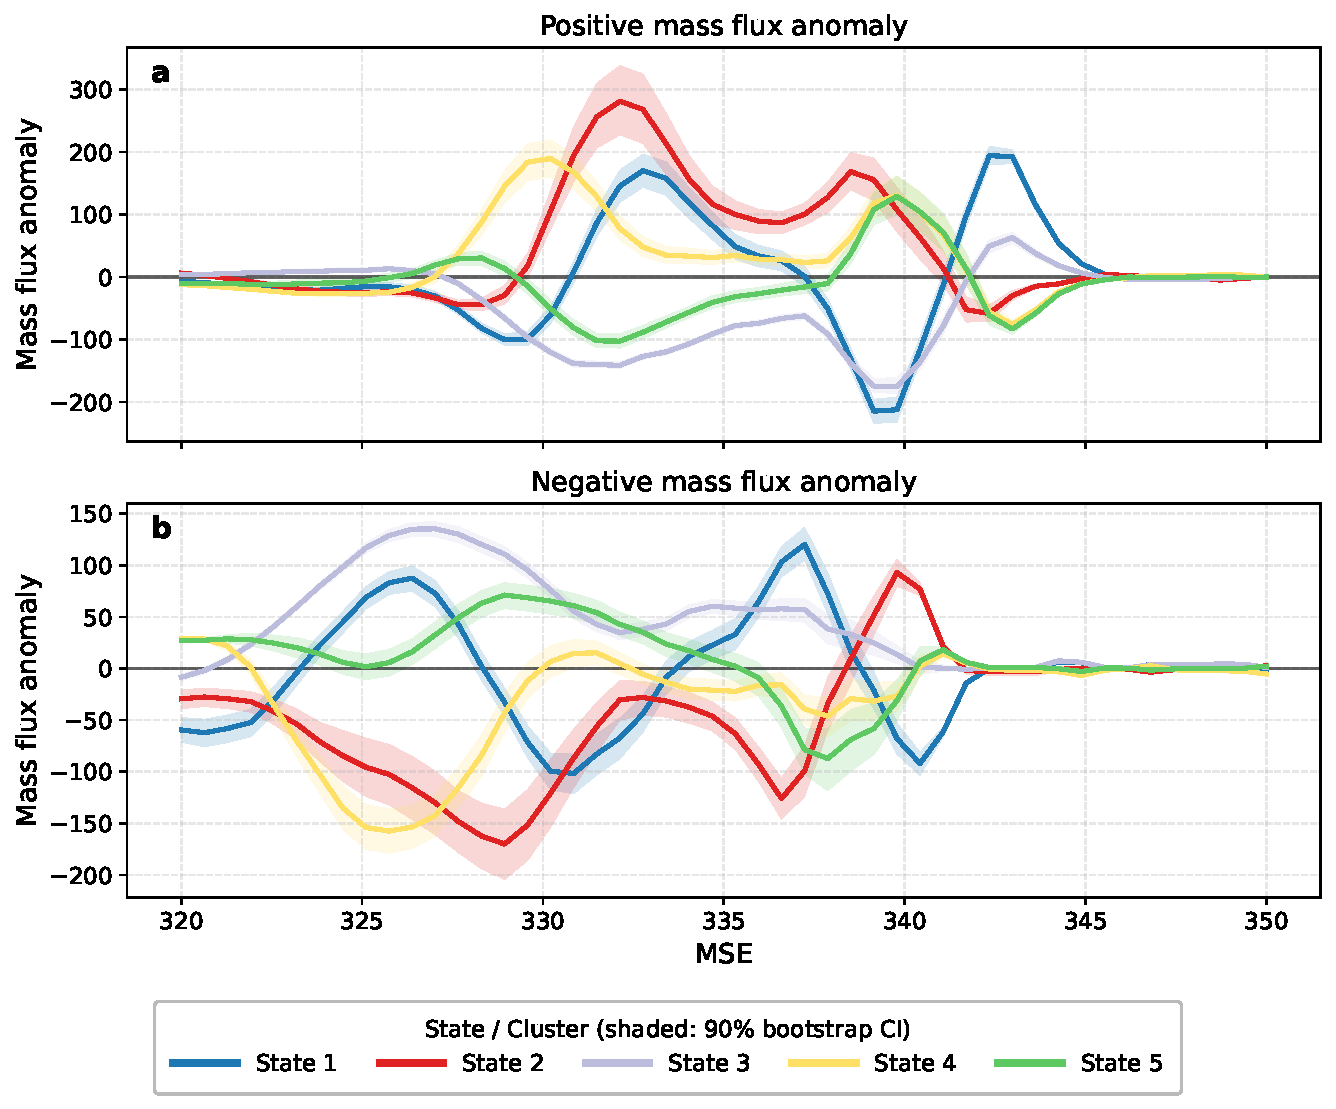
\includegraphics[width=0.72\textwidth]{fig6_mse_profiles.pdf}
    \caption{\textbf{State-averaged mass-flux anomalies resolved along moist static energy.} \textbf{(a)}~Positive (upward) and \textbf{(b)}~negative (downward) mass-flux anomalies relative to the simulation-wide mean, computed from the samples closest to each state centroid in latent space and binned by moist static energy $\theta$. Each colour corresponds to one state (see legend); solid lines indicate the per-cluster mean, and shaded bands show the 90\% bootstrap confidence interval. A peak at a given $\theta$ identifies the moist-static-energy range across which the cluster's mass-flux activity is concentrated.}
    \label{fig:mse_profiles}
\end{figure}


\section{Canonical representations of latent states}

In order to define a canonical physical representation for each latent state, we construct state-conditional mean fields using the most representative samples associated with that state. Specifically, for each state, we identify a subset of samples closest to the state barycenter in the reduced PCA–latent space and use these samples as representative realizations of the corresponding dynamical regime.

For the isentropic mass flux, we compute the mean physical field $\langle x \rangle$ by averaging the selected representative samples directly in data space. In parallel, we compute the mean latent embedding $\langle z \rangle$ over the same samples and decode it using the trained decoder, yielding $\mathrm{Dec}(\langle z \rangle)$. These two constructions correspond respectively to averaging in physical space and averaging in latent space.

Figure~\ref{fig:state_means} shows that $\langle x \rangle$ and $\mathrm{Dec}(\langle z \rangle)$ provide consistent canonical representations of each latent state. Their close agreement indicates that the latent space organizes samples in a physically meaningful manner, such that state-specific structures are preserved under both averaging procedures. As expected for a variational autoencoder, the decoded representations exhibit a mild smoothing relative to the direct physical averages, while retaining the dominant vertical and isentropic patterns characteristic of each state.

To further illustrate the physical coherence of the latent states, we also show multi-variable canonical composites constructed by averaging additional atmospheric fields over the same representative samples for each state (Fig.~\ref{fig:state_multivar}).


\begin{figure}
    \centering
    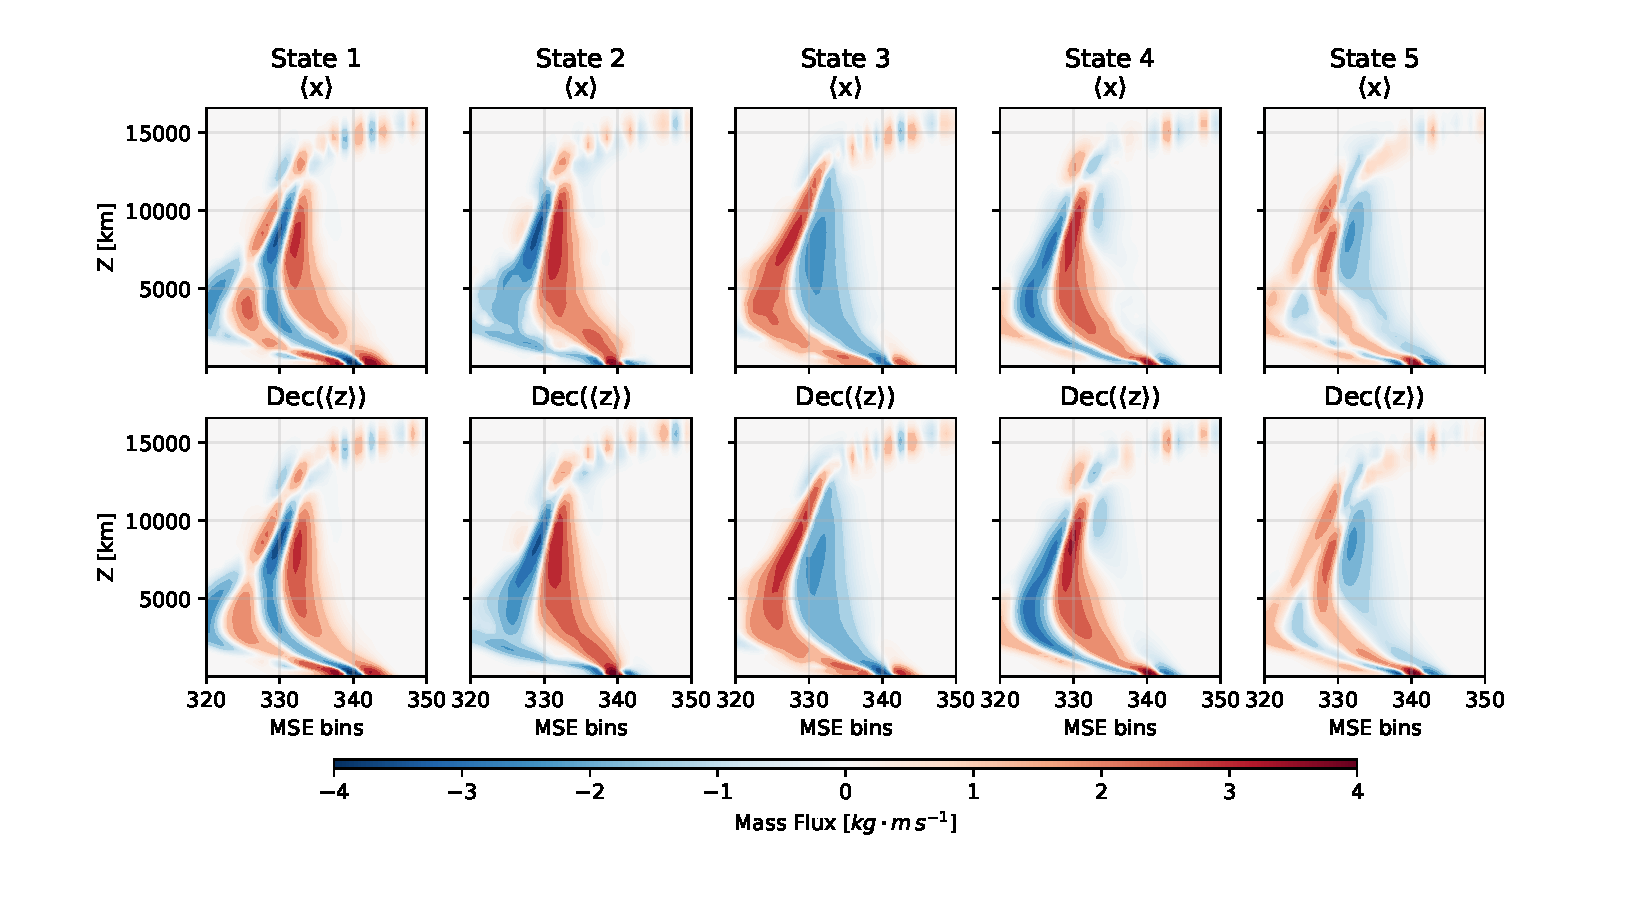
\includegraphics[width=\textwidth]{canonical_representative.pdf}
    \caption{Canonical isentropic mass flux representations for each latent state.
    Each column corresponds to a latent state, using the most representative samples closest to the state barycenter in latent space. The top row shows the mean mass flux field obtained by averaging these samples directly in physical space ($\langle x \rangle$), while the bottom row shows the reconstruction obtained by decoding the mean latent embedding of the same samples ($\mathrm{Dec}(\langle z \rangle)$). The close agreement between the two representations demonstrates that averaging in physical space and averaging in latent space yield consistent canonical state patterns, with the reconstructed fields exhibiting the characteristic smoothing expected from a variational autoencoder.}
    \label{fig:state_means}
\end{figure}


\begin{figure}
    \centering
    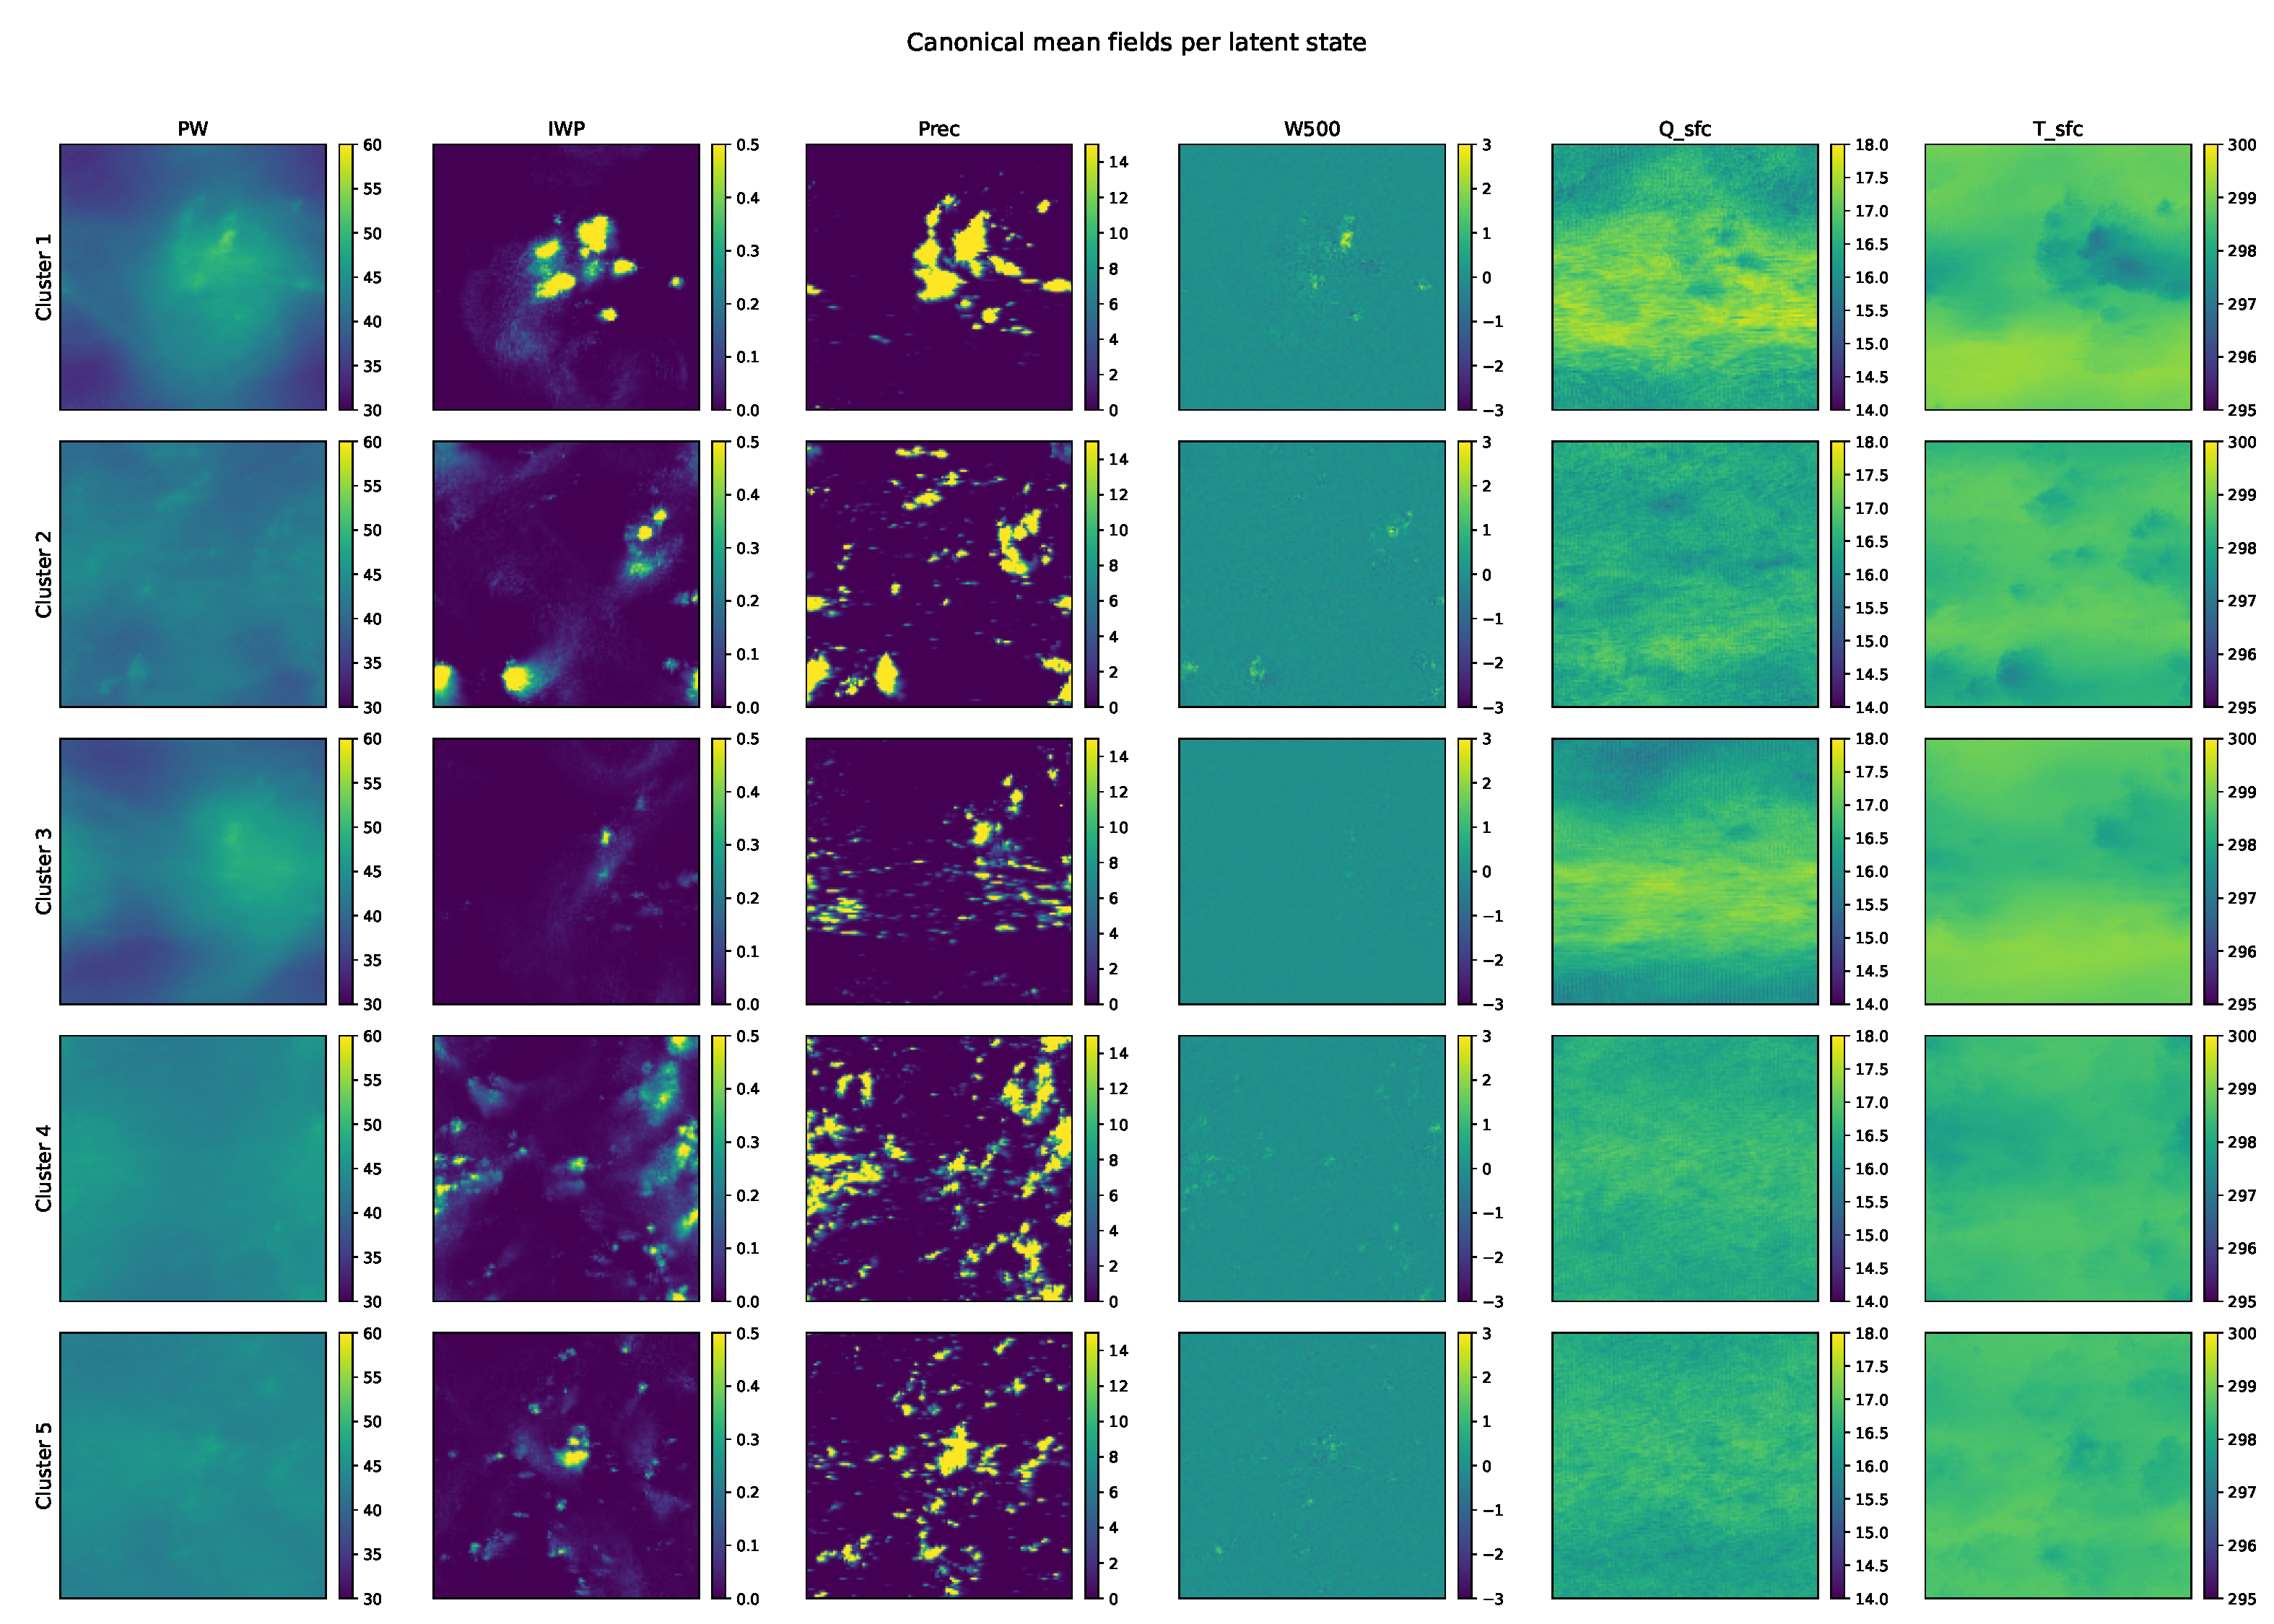
\includegraphics[width=\textwidth]{fields_clusters.pdf}
    \caption{Canonical composite fields for multiple atmospheric variables conditioned on latent states.
    For each latent state (rows), we show mean spatial fields of selected atmospheric variables (columns), computed by averaging the representative samples closest to the state barycenter in latent space. These composites provide a multi-variable physical characterization of each latent state and illustrate that the states correspond to coherent and distinct dynamical regimes.}
    \label{fig:state_multivar}
\end{figure}


\section{Cold pools tracking and activity index}
\subsection*{Cold-pool detection}

Cold pools are detected independently at each model time step from two-dimensional surface temperature field
$T_{abs}(x,y,t)$. The field is first smoothed using a Gaussian filter with standard deviation
$\sigma = 2$--$3$ grid points. Two thresholds are then applied to distinguish cold-pool envelopes and
cores. Grid points satisfying
\begin{equation}
T_{abs}(x,y,t) < \phi_{\mathrm{env}}
\end{equation}
define candidate cold-pool envelopes, while points satisfying
\begin{equation}
T_{abs}(x,y,t) < \phi_{\mathrm{core}}, \qquad \phi_{\mathrm{core}} < \phi_{\mathrm{env}},
\end{equation}
define cold-pool cores.

Envelope grid points are grouped into spatially connected objects using single-linkage agglomerative
clustering with a periodic distance metric to account for domain periodicity. Within each envelope,
core grid points are further clustered using the same approach. Core labels are subsequently propagated
to the surrounding envelope using nearest-neighbor classification, yielding a fully labeled cold-pool
mask at each time step.


\subsection*{Temporal tracking}

Cold-pool objects are tracked forward in time by matching labeled regions between consecutive time
steps based on spatial overlap. For a cold pool with label $i$ at time $t$ and label $j$ at time $t+1$,
the similarity is defined as
\begin{equation}
S_{ij} = \frac{|A_i(t) \cap A_j(t+1)|}{|A_i(t)|},
\end{equation}
where $A_i(t)$ denotes the set of grid points belonging to object $i$ at time $t$. Labels are
propagated when $\max_j S_{ij} > 0.55$, ensuring temporal continuity while allowing for cold-pool
initiation, dissipation, splitting, and merging.

\subsection*{Object-based diagnostics}

Tracked cold pools are characterized using near-surface specific humidity $q_v(x,y,t)$. For each cold
pool $k$ at time $t$, the mean humidity anomaly is defined as
\begin{equation}
\Delta q_v^k(t) = \langle q_v \rangle_k(t) - \langle q_v \rangle_{\mathrm{domain}}(t),
\end{equation}
where angle brackets denote spatial averaging over the cold-pool area and the full domain,
respectively. For each cold pool, we record its lifetime, time-evolving area $A_k(t)$, maximum area,
mean humidity anomaly over its lifetime, and maximum absolute humidity anomaly.

\subsection*{Cold-pool index}

A Cold-Pool Index (CPI) is defined as the total area covered by cold pools at each time step,
\begin{equation}
\mathrm{CPI}(t) = \sum_k A_k(t),
\end{equation}
where the sum is taken over all cold pools present at time $t$. In addition to the raw CPI, normalized,
anomalous, and standardized versions are computed using the temporal mean and standard deviation.


\section{Autocorrelation of state indicators in a Markov chain}

Let $\{X_t\}_{t\ge 0}$ be a discrete-time, stationary Markov chain on a finite
state space $\{1,\dots,K\}$ with transition matrix $\mathbf{T}$ and stationary
distribution $\boldsymbol{\pi}$, satisfying
\begin{equation}
    \mathbf{T}\boldsymbol{\pi} = \boldsymbol{\pi},
    \qquad
    \sum_{i=1}^K \pi_i = 1,
    \qquad
    \pi_i \ge 0.
\end{equation}

For a given state $i$, we define the state indicator function
\begin{equation}
    I_i(t) = \mathbb{1}[X_t = i].
\end{equation}
Under stationarity, its expectation is
\begin{equation}
    \mathbb{E}[I_i(t)] = \mathbb{P}(X_t = i) = \pi_i.
\end{equation}

We define the normalized autocorrelation function
\begin{equation}
    C_i(\tau)
    =
    \frac{
        \mathbb{E}\!\left[(I_i(t)-\pi_i)(I_i(t+\tau)-\pi_i)\right]
    }{
        \mathbb{E}\!\left[(I_i(t)-\pi_i)^2\right]
    }.
\end{equation}

\paragraph{Denominator.}
Since $I_i(t)$ is a Bernoulli random variable,
\begin{equation}
    \mathbb{E}\!\left[(I_i(t)-\pi_i)^2\right]
    = \pi_i(1-\pi_i).
\end{equation}

\paragraph{Numerator.}
Expanding the expectation,
\begin{equation}
\begin{aligned}
    \mathbb{E}\!\left[(I_i(t)-\pi_i)(I_i(t+\tau)-\pi_i)\right]
    &=
    \mathbb{E}[I_i(t)I_i(t+\tau)] - \pi_i^2.
\end{aligned}
\end{equation}

By stationarity and the Markov property,
\begin{equation}
    \mathbb{E}[I_i(t)I_i(t+\tau)]
    =
    \mathbb{P}(X_t=i, X_{t+\tau}=i)
    =
    \pi_i (\mathbf{T}^\tau)_{ii}.
\end{equation}

Therefore,
\begin{equation}
    \mathbb{E}\!\left[(I_i(t)-\pi_i)(I_i(t+\tau)-\pi_i)\right]
    =
    \pi_i \left[(\mathbf{T}^\tau)_{ii} - \pi_i \right].
\end{equation}

\paragraph{Autocorrelation expression.}
Combining numerator and denominator yields
\begin{equation}
    C_i(\tau)
    =
    \frac{(\mathbf{T}^\tau)_{ii} - \pi_i}{1-\pi_i}.
\end{equation}

\paragraph{Spectral decomposition.}
Let the eigenvalues of $\mathbf{T}$ be $(1,\lambda_2,\dots,\lambda_K)$, where
$\lambda_1=1$ corresponds to the stationary mode and
$|\lambda_\alpha|<1$ for $\alpha\ge2$.
Using the spectral decomposition,
\begin{equation}
    \mathbf{T}^\tau
    =
    \mathbf{1}\boldsymbol{\pi}^\top
    + \sum_{\alpha=2}^K \lambda_\alpha^\tau
    \mathbf{v}_\alpha \mathbf{w}_\alpha^\top,
\end{equation}
where $\mathbf{v}_\alpha$ and $\mathbf{w}_\alpha$ are the right and left
eigenvectors of $\mathbf{T}$, respectively.

Substituting into the expression for $C_i(\tau)$, the stationary contribution
cancels exactly, yielding
\begin{equation}
    C_i(\tau)
    =
    \sum_{\alpha=2}^K
    A_\alpha^{(i)} \lambda_\alpha^\tau,
\end{equation}
with coefficients
\begin{equation}
    A_\alpha^{(i)}
    =
    \frac{
        (\mathbf{v}_\alpha)_i (\mathbf{w}_\alpha)_i
    }{
        1-\pi_i
    }.
\end{equation}

\paragraph{Asymptotic behavior.}
At large time lags, the autocorrelation is dominated by the second-largest
eigenvalue,
\begin{equation}
    C_i(\tau) \sim \lambda_2^\tau
    =
    \exp\!\left(-\tau / \tau_{\mathrm{corr}}\right),
\end{equation}
where the correlation time is
\begin{equation}
    \tau_{\mathrm{corr}} = -\frac{1}{\ln|\lambda_2|}.
\end{equation}

Exponential decay of state autocorrelations is therefore a direct consequence
of the Markov property.


\bibliographystyle{apsrev4-2}
\bibliography{biblio}

\end{document}